\documentclass[10pt, a4paper]{article}
\usepackage{amsmath}
\usepackage{tikz}
\usetikzlibrary{shadows}
\usetikzlibrary{arrows}
\usepackage{colortbl}

\begin{document}

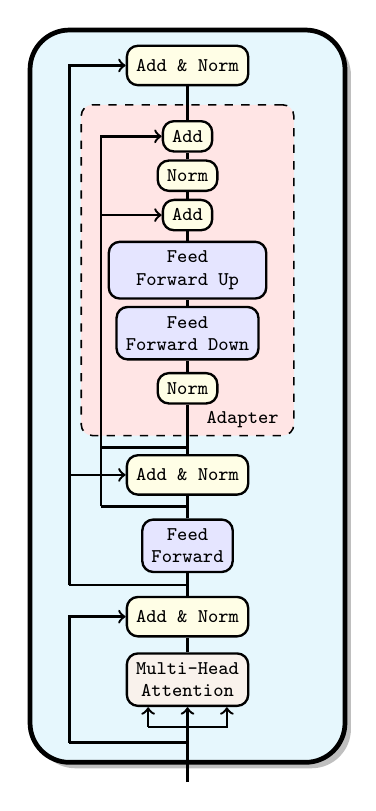
\begin{tikzpicture}[block/.style={rectangle, draw, line width=0.3mm, rounded corners, font=\ttfamily\scriptsize}]
    \node[block, minimum width=4.0cm, minimum height=9.3cm, line width=0.6mm, rounded corners=5mm, fill=cyan!10, drop shadow] (main) at (0,-0.6) {};
    \node[block, dashed, minimum width=2.7cm, minimum height=4.2cm, line width=0.2mm, fill=red!10] (main) at (0,1.0) {};

    \node[block, minimum width=1cm, minimum height=0.5cm, line width=0.3mm, align=center, fill=yellow!10] (add3) at (0, 3.6) {Add \& Norm};

    \node[block, draw, minimum width=0.5cm, minimum height=0.2cm, line width=0.3mm, align=center, fill=yellow!10] (addadap2) at (0,2.7) {Add};
    \node[block, draw, minimum width=0.5cm, minimum height=0.2cm, line width=0.3mm, align=center, fill=yellow!10] (normadap2) at (0,2.2) {Norm};
    \node[block, draw, minimum width=0.5cm, minimum height=0.2cm, line width=0.3mm, align=center, fill=yellow!10] (addadap1) at (0,1.7) {Add};

    \node[block, minimum width=2cm, minimum height=0.5cm, line width=0.3mm, align=center, fill=blue!10] (ff3) at (0,1.0) {Feed \\ Forward Up};
    \node[block, minimum width=1cm, minimum height=0.5cm, line width=0.3mm, align=center, fill=blue!10] (ff2) at (0,0.2) {Feed \\ Forward Down};
    \node[block, draw, minimum width=0.5cm, minimum height=0.2cm, line width=0.3mm, align=center, fill=yellow!10] (normadap1) at (0,-0.5) {Norm};


    \node[block, minimum width=1cm, minimum height=0.5cm, line width=0.3mm, align=center, fill=yellow!10] (add2) at (0,-1.6) {Add \& Norm};
    \node[block, minimum width=1cm, minimum height=0.5cm, line width=0.3mm, align=center, fill=blue!10] (ff1) at (0,-2.5) {Feed \\ Forward};
    \node[block, minimum width=1cm, minimum height=0.5cm, line width=0.3mm, align=center, fill=yellow!10] (add1) at (0,-3.4) {Add \& Norm};
    \node[block, minimum width=1cm, minimum height=0.5cm, line width=0.3mm, align=center, fill=brown!10] (att1) at (0,-4.2) {Multi-Head \\ Attention};

    \draw[->, line width=0.3mm] (-1.1,-2.0) |- (addadap2);
    \draw[->, line width=0.3mm] (-1.1,-2.0) |- (addadap1);

    \draw[line width=0.3mm] (0,-2.0) |- (-1.1,-2.0);
    \draw[line width=0.3mm] (0,-1.25) |- (-1.1,-1.25);


    \draw[->, line width=0.3mm] (-1.5,-3.0) |- (add3);

    \draw[->, line width=0.3mm] (-1.5,-3.0) |- (add2);
    \draw[line width=0.3mm] (0,-3.0) |- (-1.5,-3.0);

    \draw[->, line width=0.3mm] (-1.5,-5.0) |- (add1);
    \draw[line width=0.3mm] (0,-5.0) |- (-1.5,-5.0);

    \draw[->, line width=0.3mm] (-0.5,-4.8) -| (0.5, -4.55);
    \draw[->, line width=0.3mm] (-0.5,-4.8) -| (-0.5, -4.55);
    \draw[->, line width=0.3mm] (0,-5.5) -- (-0,-4.55);


    \path[every node/.style={font=\sffamily\small}]
        (att1) edge[line width=0.3mm] node [right] {} (add1)
        (add1) edge[line width=0.3mm] node [right] {} (ff1)
        (ff1) edge[line width=0.3mm] node [right] {} (add2)
        (add2) edge[line width=0.3mm] node [right] {} (normadap1)
        (normadap1) edge[line width=0.3mm] node [right] {} (ff2)
        (ff2) edge[line width=0.3mm] node [right] {} (ff3)
        (ff3) edge[line width=0.3mm] node [right] {} (addadap1)
        (addadap1) edge[line width=0.3mm] node [right] {} (normadap2)
        (normadap2) edge[line width=0.3mm] node [right] {} (addadap2)
        (addadap2) edge[line width=0.3mm] node [right] {} (add3);


    \node[font=\scriptsize\ttfamily\bfseries, text centered, text width=1cm] at (0.7,-0.9) {Adapter};


\end{tikzpicture}

\end{document}